%% Background
\chapter{Background}
\label{chap:background}

\section{Font Selection}

\subsection{Current Font Selection Tools}

\begingroup
\parfillskip=0pt

Surprisingly little progress has been made in the past several decades on the issue of user font selection. When a user searches for a new font, almost every major word processor presents them with the same interface: a basic, linear list of typefaces with some additional controls over parameters like size, weight, and underline. This interface is essentially the same as those used in the earliest multi-font

\par
\endgroup

% from Designing the Xerox “Star” User Interface, Byte, issue 4, 1982
\begin{figure}[H]
    \centering
    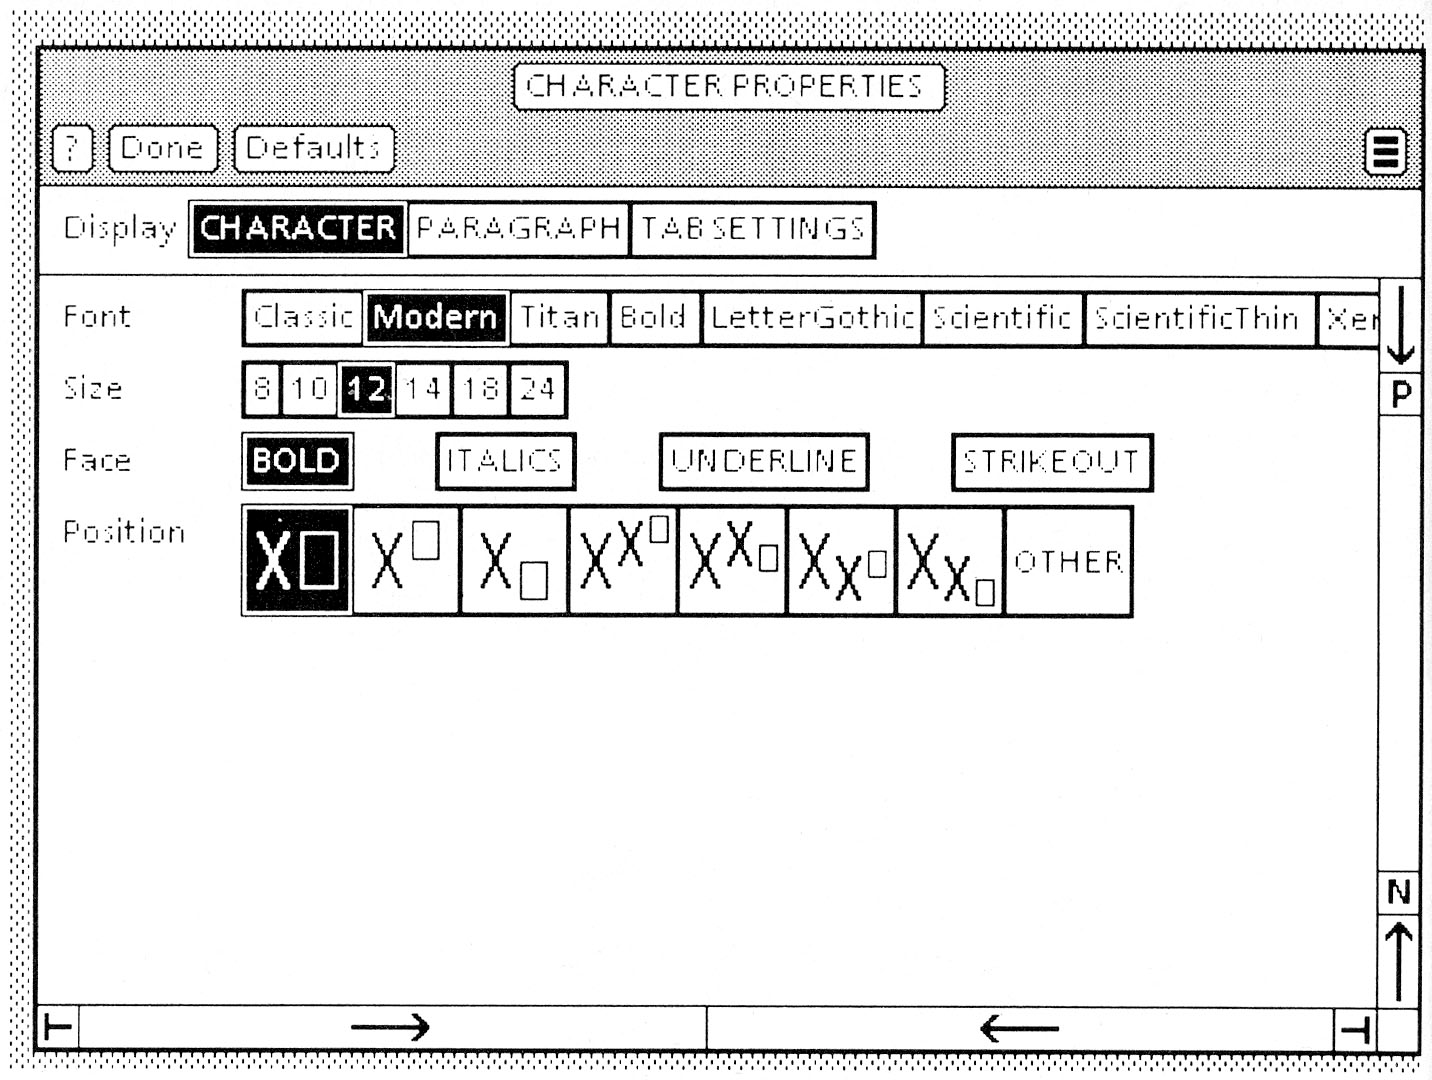
\includegraphics[width=.8\textwidth]{images/xerox-star.png}
    \caption{Font selection interface in Xerox Star (1981)}
    \label{fig:xerox-star}
\end{figure}

% own screenshots
\begin{figure}[H]
    \centering
    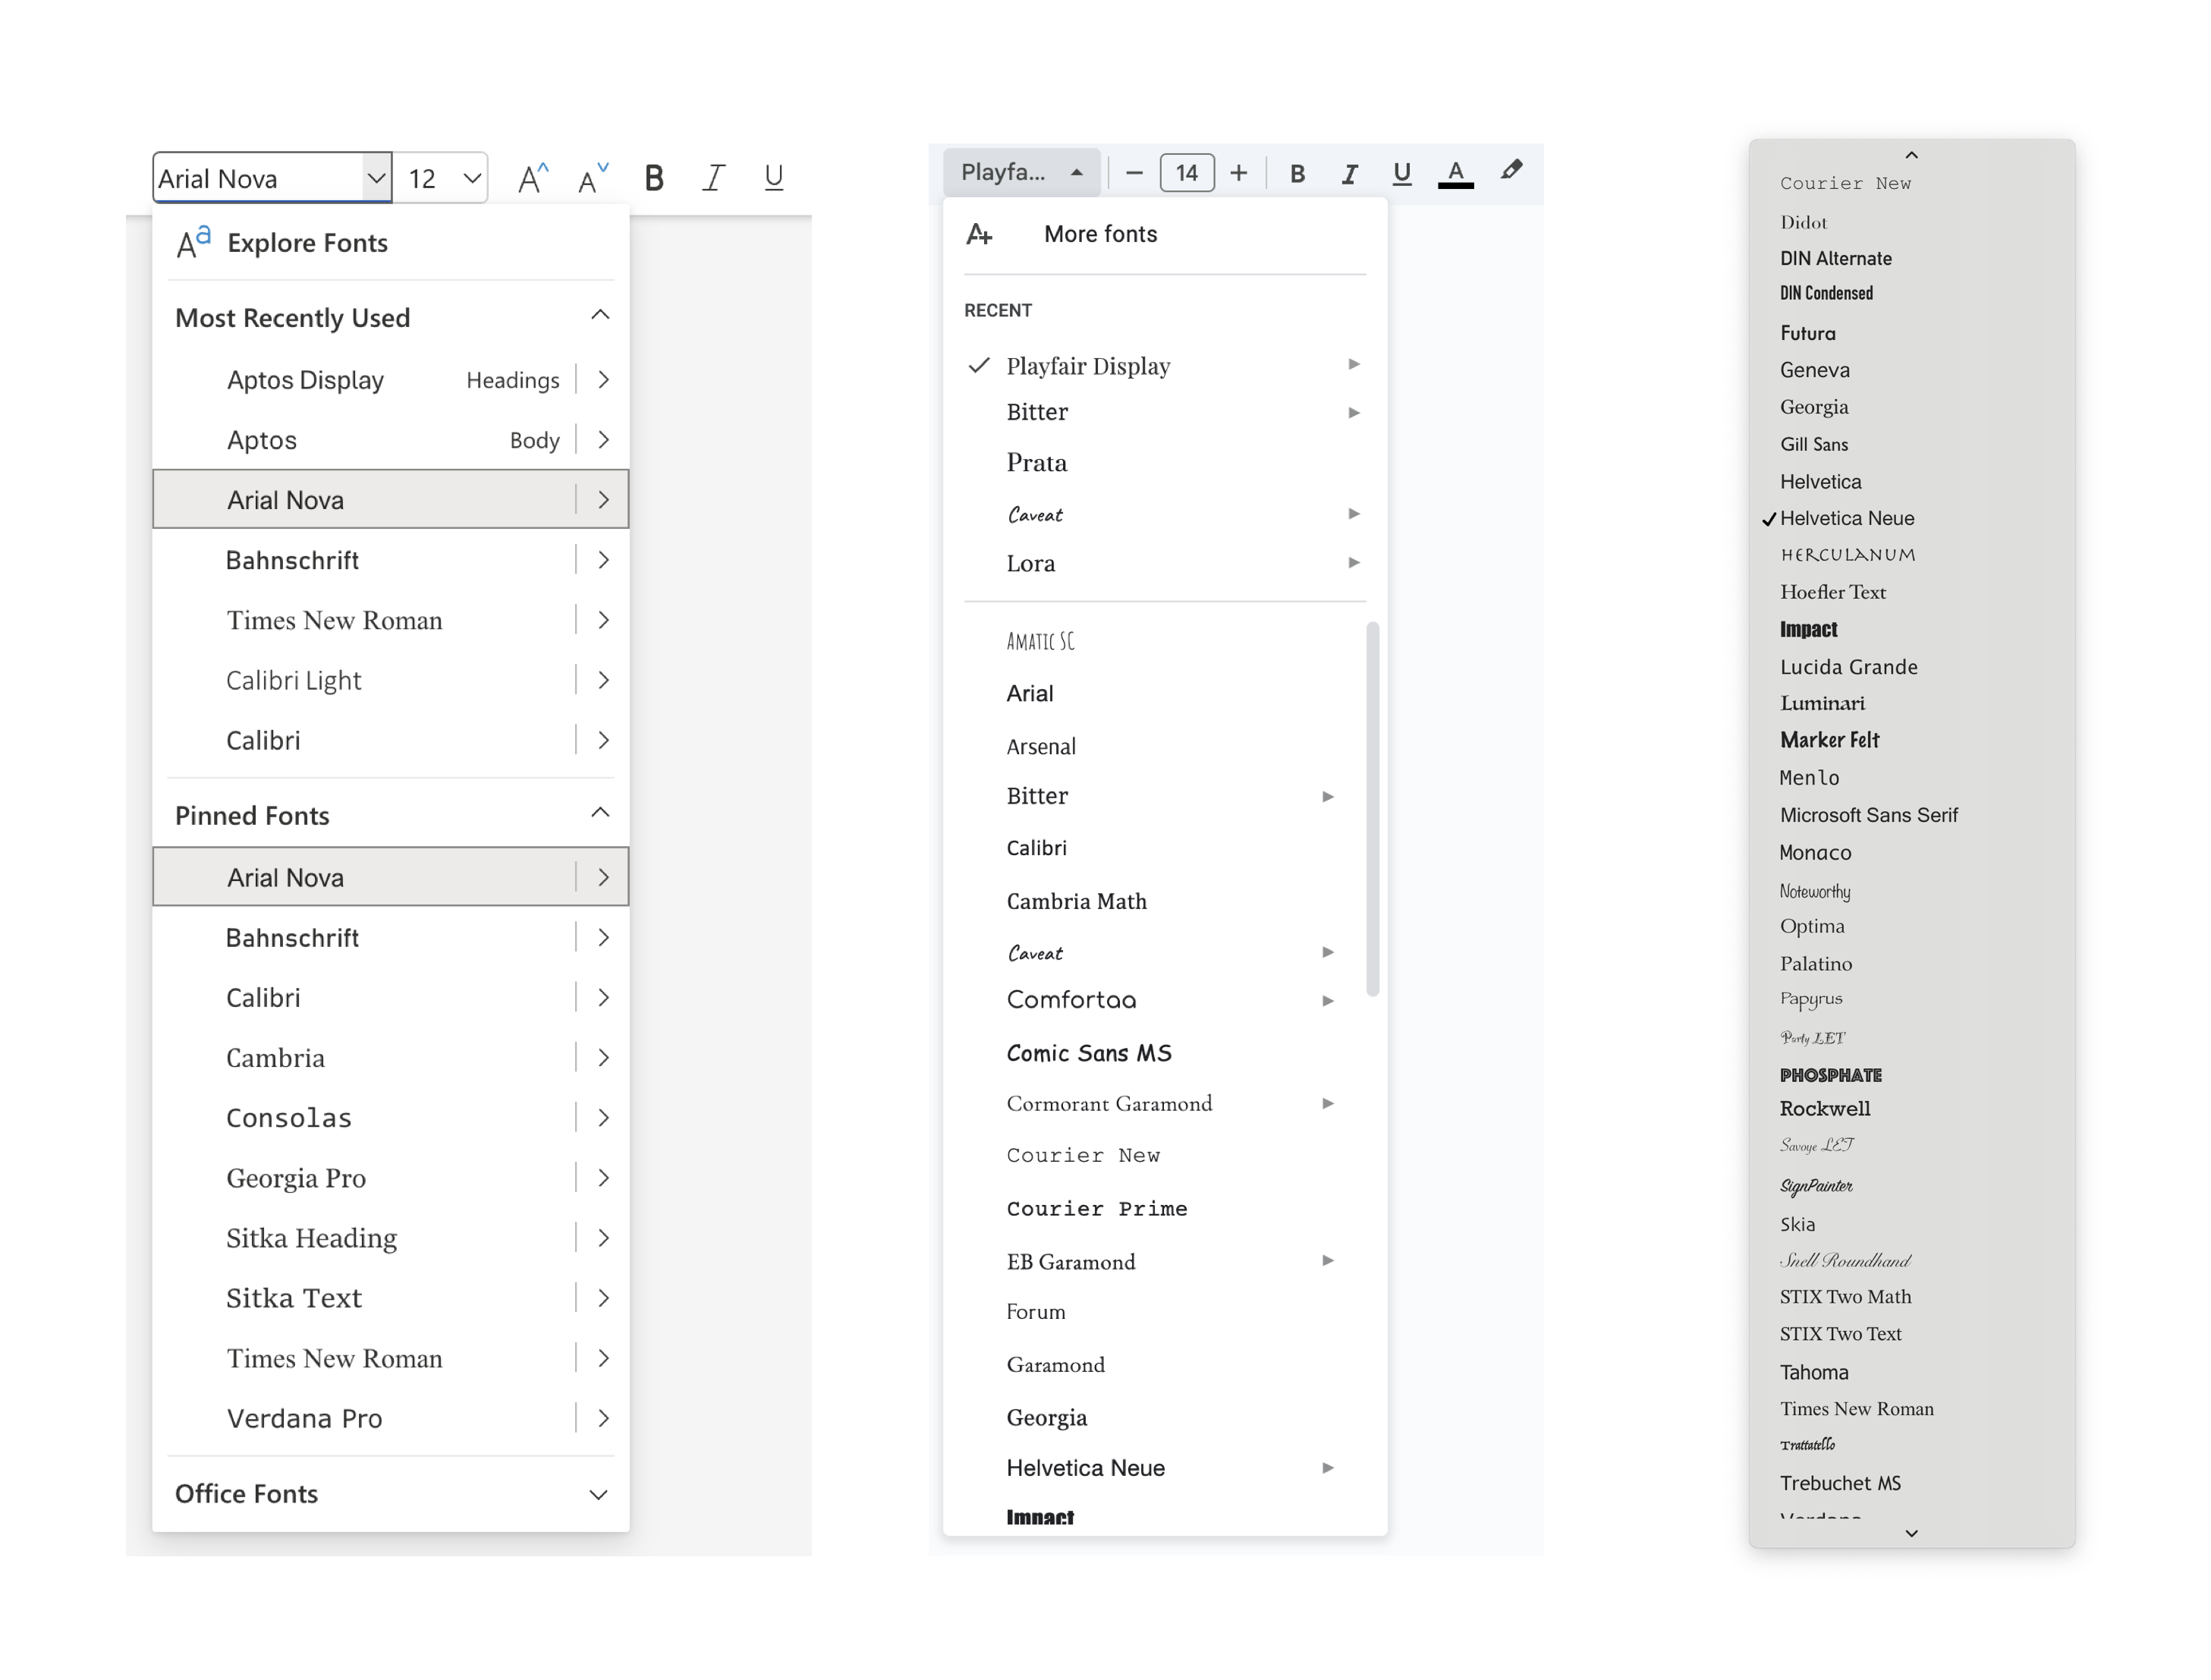
\includegraphics[width=1\textwidth]{images/font-selectors.png}
    \caption{Current font selection interfaces in Microsoft Word, Google Docs, and Apple Pages}
    \label{fig:font-selectors}
\end{figure}

\noindent word processors (see Figures \ref{fig:xerox-star} and \ref{fig:font-selectors}), and it offers users little support or guidance when making style-based decisions. Moreover, the number of fonts accessible to users has grown by several orders of magnitude: whereas early word processors contained only a handful of fonts for users to choose between, the number of individual fonts available to users now (although impossible to enumerate exactly) almost certainly exceeds 300,000 \cite{cheng2006}.

O'Donovan et al. \cite{odonovan2014} lists several reasons for the difficulty of developing font selection tools. The first issue is the sheer number of available fonts. ``Most computers are now equipped with hundreds of fonts,'' they note, while online resources provide access to hundreds of thousands. Another issue is a lack of obvious ways to categorize fonts in a manner which corresponds to user goals. While there exist broad categories like Serif, Sans Serif, and Handwritten, these must be manually designated on a per-font basis, and these categories are not necessarily helpful to every user. A thesis student, for example, might know that they should choose a Serif font for their thesis to convey an academic mood—or, more practically, to fulfill certain design expectations for their final document—however another user, perhaps a coffee shop owner deciding on a font for their shop's logo, might not find the distinction between Serif, Sans Serif, and Handwritten particularly useful, or know where to start in deciding between them. A graphic designer, who has studied typeface design for years and has relevant experience, might feel confident in handling these categorizations, but most users do not have this background. A typical user lacks the necessary tools, given the current state of font selector interfaces, to properly consider the wide range of diverse typefaces and make one of the most fundamental decisions in effective text-based graphical design. Finally, different users vary in their font selection goals. One user may be looking to match a particular font they found on a store sign or brochure—or to find a free-to-use font which is a close match to the commerical one. Another may be looking to match a particular mood, or choose a font that fits well with the rest of their document. A third may simply be exploring a large set of fonts like Adobe TypeKit or Google Fonts, curious to find their next favorite font. O'Donovan et al. argue—and we agree—that current methods of font selection fall short on these issues and more. Given the growing number of fonts available to the modern user, a better, more useful system for typeface selection is necessary.

\subsection{Font Selection Innovation}

There has been, however, some progress in recent years in the field of font selection interfaces. Specifically, both Google Fonts and Canva (a popular online graphic design tool) have experimented with language-based font selection tools. These are both interesting experiments into font selection interfaces which break from the list-based interface, but both tools fall short on several grounds.

% own screenshots
\begin{figure}[ht]
    \centering
    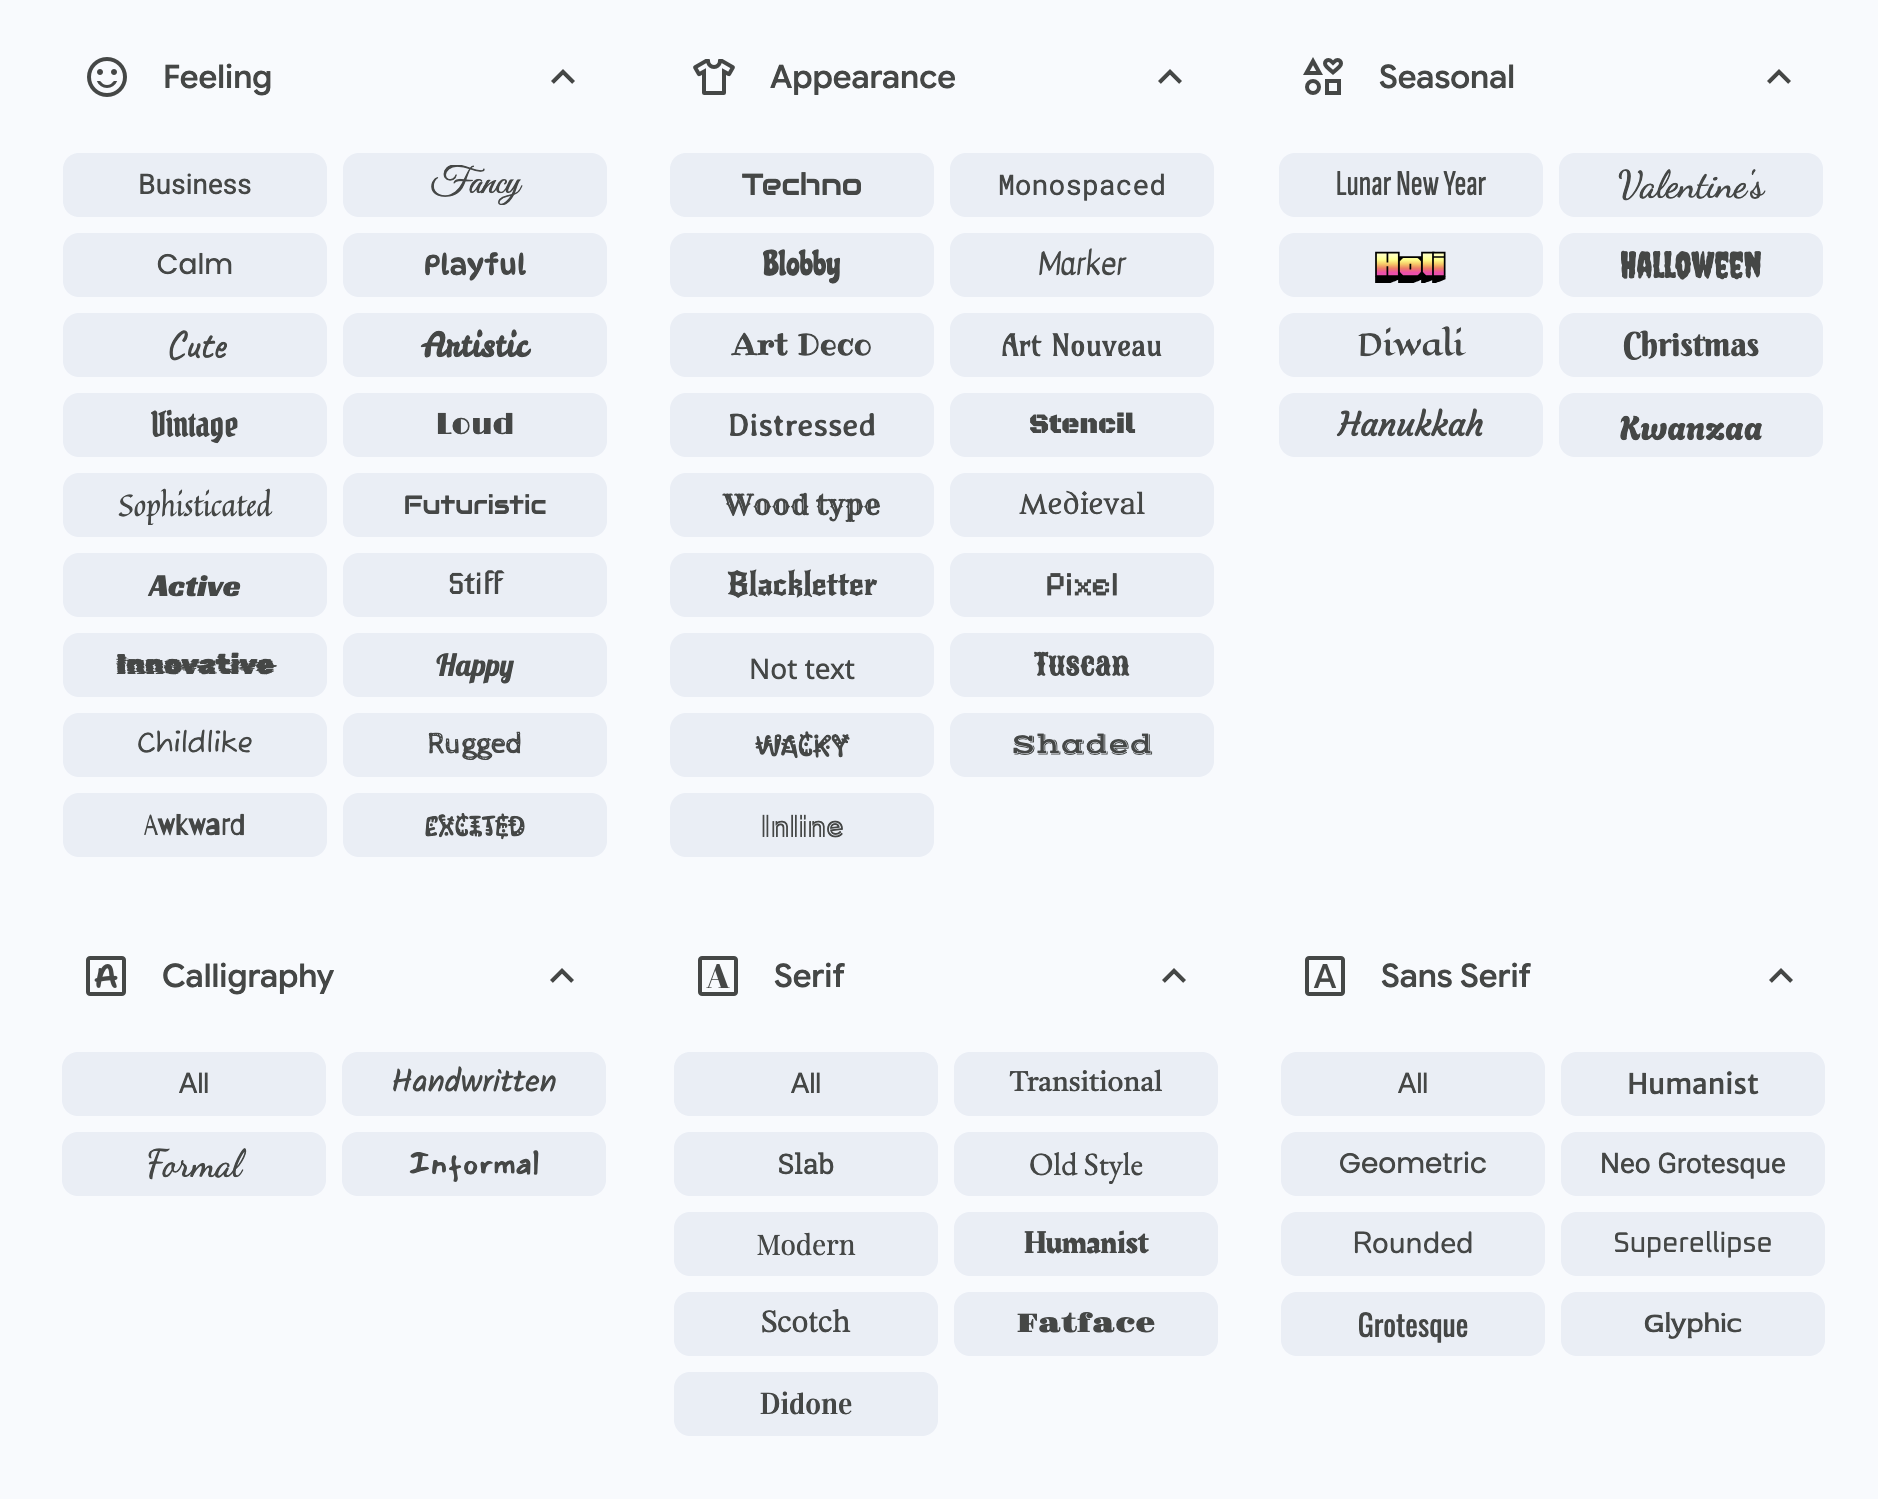
\includegraphics[width=.85\textwidth]{images/google-font-categories.png}
    \caption{Some of the new typeface categorizations from Google Fonts}
    \label{fig:google-font-categories}
\end{figure}

The new font selection interface on the Google Fonts website\footnote{https://fonts.google.com} was released around early 2025. Whereas Google previously sectioned their fonts into 5 broad categories (Display, Handwriting, Monospace, Serif, and Sans Serif), their new interface introduces many more typeface categories, broken into larger parent categories. In the ``Feeling" category, for example, users can filter ``Happy" fonts, ``Calm" or ``Playful" fonts, and ``Childlike" or ``Awkward" fonts. The new interface includes appearance categories like ``Techno" or ``Art Deco," and also holiday categories like Halloween, Hanukkah, and Holi.

% own screenshots
\begin{figure}[H]
    \centering
    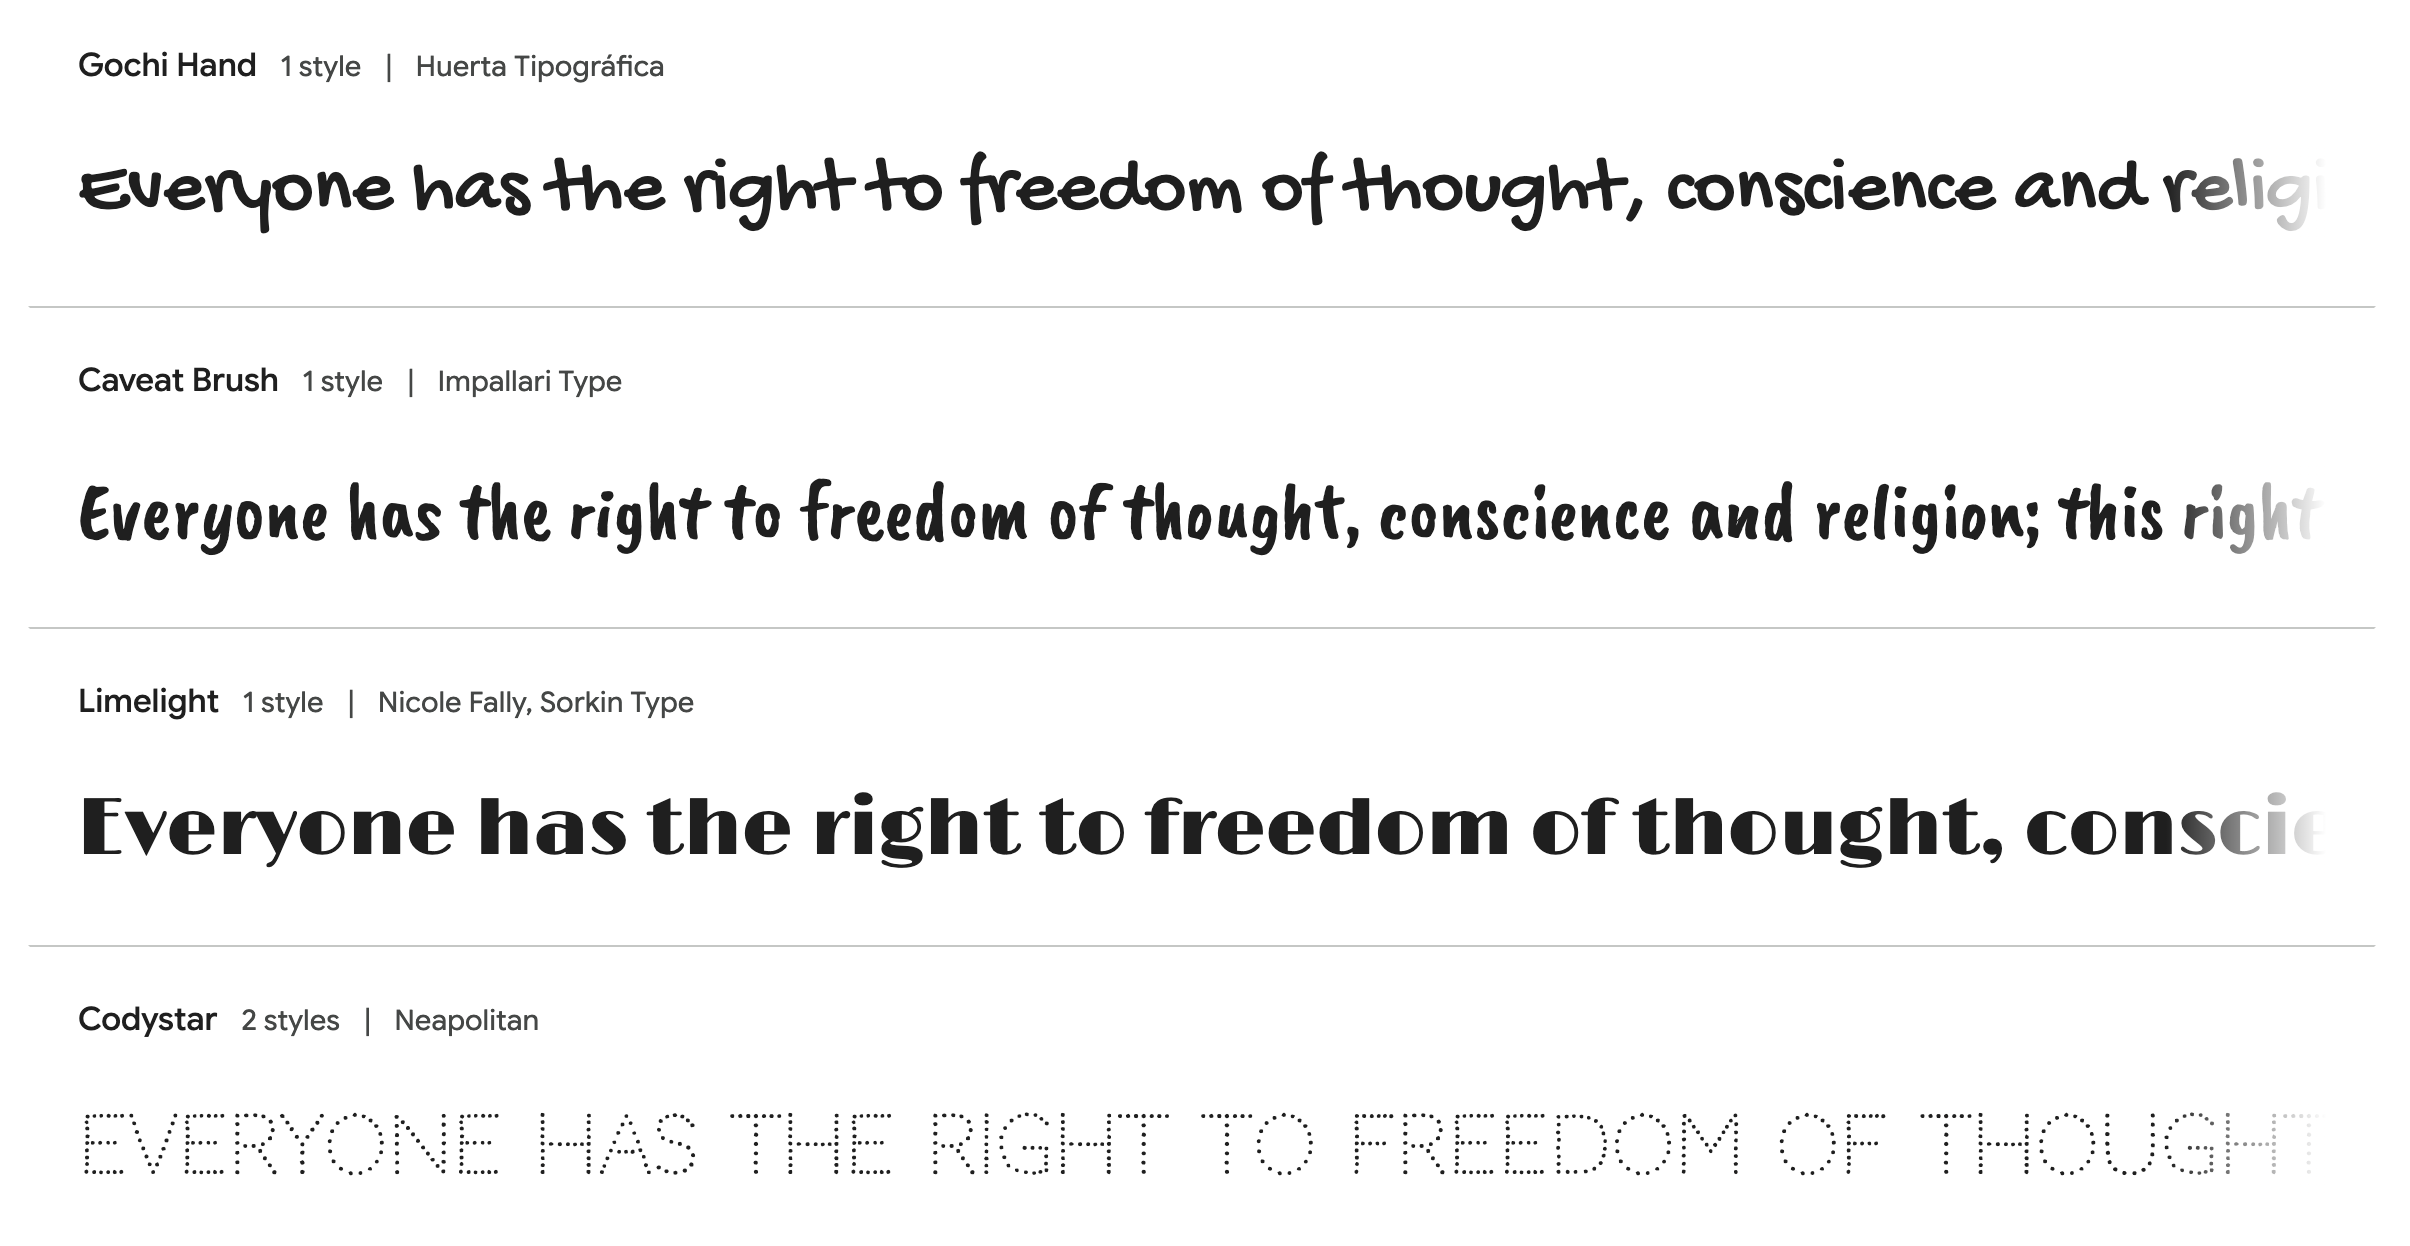
\includegraphics[width=1\textwidth]{images/google-fonts-christmas.png}
    \caption{Some of the fonts in the ``Christmas'' category of Google Fonts}
    \label{fig:google-fonts-christmas}
\end{figure}

Google Font's categories are impressive and break with typical font-selection tools; however, the tool has several drawbacks. For one, the user is forced into discrete categories, rather than an open-ended text input. Additionally, while many of the categorizations are fairly accurate, some are more questionable. (For example, see some of the fonts categorized under ``Christmas" in Figure \ref{fig:google-fonts-christmas}.) Most importantly, however, Google has not incorporated this new font selection tool into their main Google Suite applications (Google Docs, Google Slides, and Google Sheets) where the majority of their users require assistance in font selection. This new font selector tool, available only from a separate website, appears to be an interesting experiment but not much more than that.

Canva, a popular online graphic design tool, has also experimented with a language-based font selection tool: their main design interface allows users access to a font-selector tool with a text input field. A user could type ``Modern'' and they would be presented with a wide-variety of modern-style fonts. However, while the tool seems to be open-ended, it actually only works for a small set of keywords; for most text input, the tool will either yield no results, or will simply return fonts whose name contains that keyword. (See Figure \ref{fig:canva-font-selector} for some usage examples.) For example, the Canva tool will return no results for inputs like ``Professional,'' ``Cheerful,'' or ``Hanukkah.'' As with the new Google Fonts category-based selector, this font selection interface seems appears more of an experiment than a user-ready tool.

% own screenshots
\begin{figure}
    \centering
    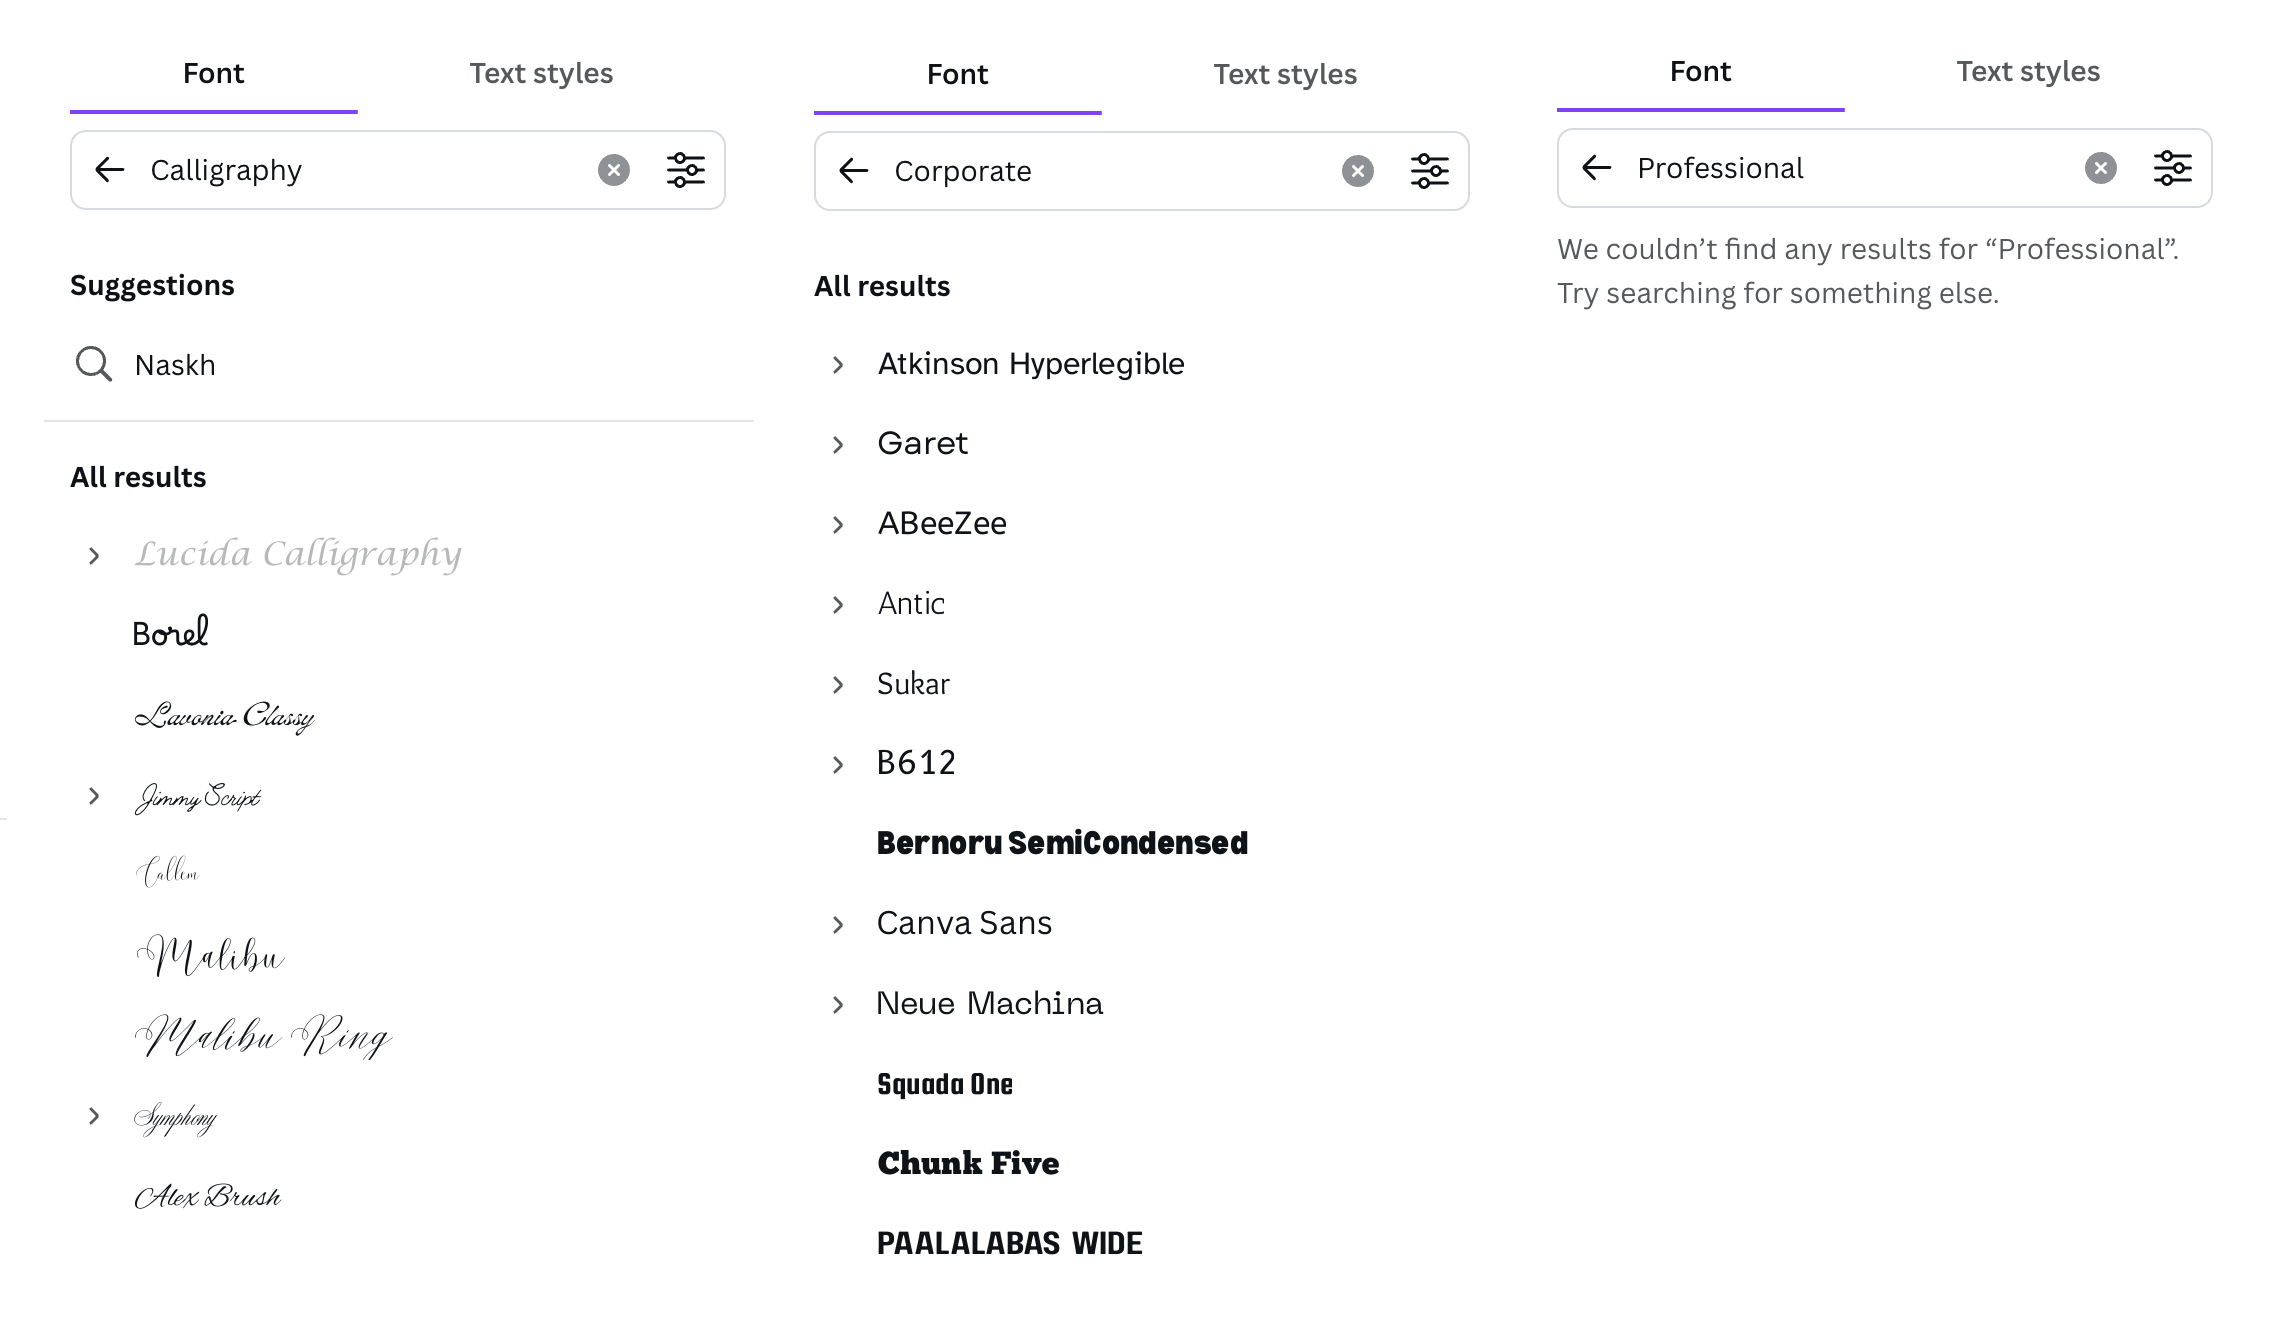
\includegraphics[width=.95\textwidth]{images/canva-font-selector.png}
    \caption{Example usages of the Canva text-based font selector tool}
    \label{fig:canva-font-selector}
\end{figure}

\subsection{Issues with Language-Based Models}

where is the labelled data??

\section{Autoencoders}

As previously stated, we hypothesize that neural networks might provide a useful foundation for font selection tools by generating typeface style encodings. More specifically, we focus on autoencoder and autoencoder-like models in our neural network design. This section, therefore, provides necessary background on the autoencoder model and why autoencoder-like neural networks might provide a useful foundation for style-based font selection tools.

\subsection{Autoencoder Model}

The autoencoder, originally proposed by Rumelhart et al. \cite{rumelhart1986}, is a specific type of neural network trained to exactly reconstruct its own input data. The model is composed of two parts: an encoder, which transforms the input data to an intermediate representation (usually smaller than the input data) through a series of linear and nonlinear layers; and the decoder, which similarly transforms the intermediate representation to the original input size. By minimizing the loss of this neural network during training, the autoencoder learns to reconstruct input data.

% from Bank et al. "Autoencoders" DO I NEED TO CITE THIS?
\begin{figure}[h]
    \centering
    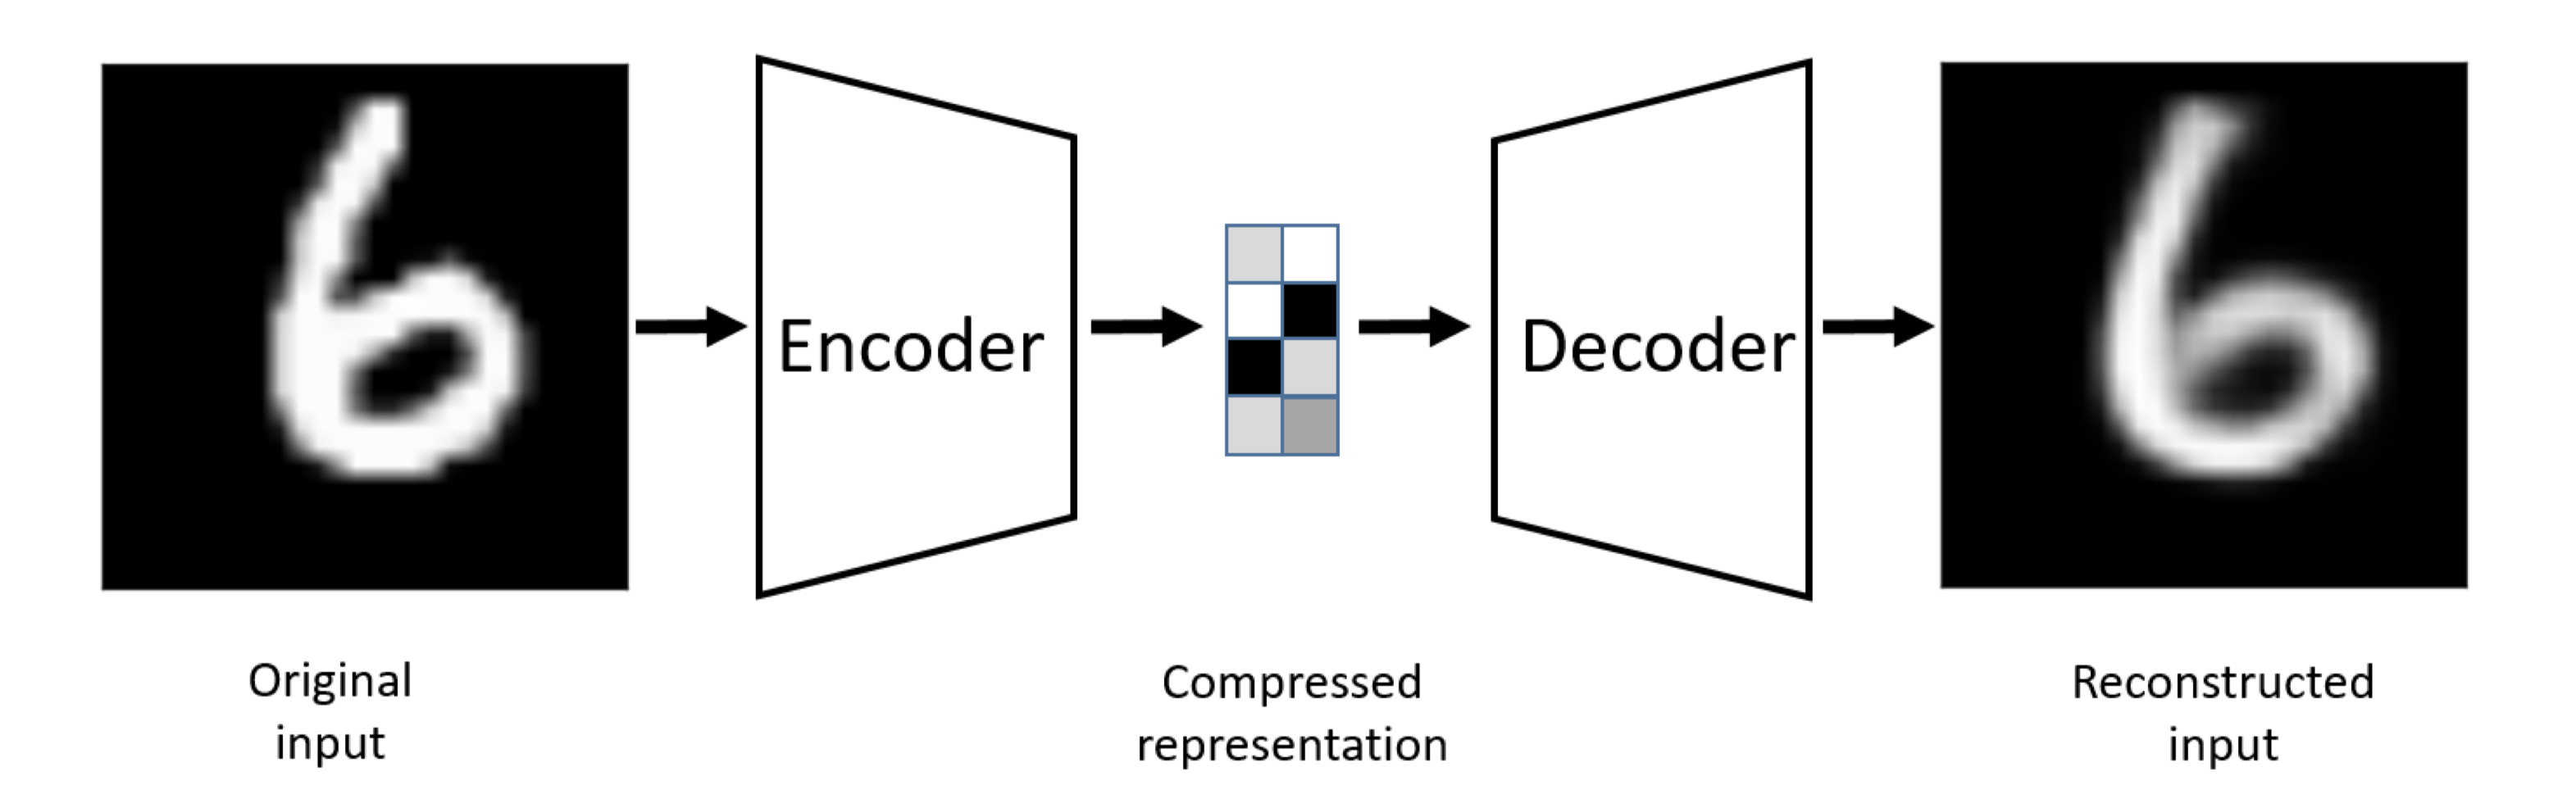
\includegraphics[width=\textwidth]{images/autoencoder-model.png}
    \caption{Basic autoencoder model applied on MNIST data}
    \label{fig:autoencoder-model}
\end{figure}

\noindent One main goal of the autoencoder is to distill a meaningful representation of the input data, which might represent something intrinsic about the data. (In our case, this meaningful representation would be the typeface style.) In their well-known chapter on autoencoders, Bank et al. write:

\begin{quote}
    ...the goal of autoencoders is to get a compressed and meaningful
    representation. We would like to have a representation that is meaningful to us... \cite{bank2021autoencoders}
\end{quote}

\noindent In order to create these meaningful representations, however, some some steps must be taken to avoid simply learning the identity function. Usually this is accomplished by virtue of the model's bottleneck—assuming the intermediate representation is smaller than the input data—but other methods such as adding Gaussian noise can also be used to achieve this regularization.

\subsection{Autoencoder Variations}

There have been many variations on this basic autoencoder model to prioritize different model goals. While the basic autoencoder is unsupervised, it is possible to feed additional data into the autoencoder, such as data labels, in order to coerce the model to ignore these aspects of the input data in the construction of an intermediate representation. (In our research, we employ this method to disentangle \textit{letter} meaning from \textit{style} meaning.) Another alteration of the original autoencoder is the variational autoencoder (VAE) model introduced by Kingma et al. \cite{kingma2013}, which uses probabilistic distributions to improve the autoencoder model, especially with respect to generative tasks. Rather than encoding an explicit intermediate encoding, VAEs encode the parameters of a multi-dimensional Gaussian distribution from which the decoder samples before the decoding task. This is especially useful in generative tasks, when the goal is to generate new data, but the continuous latent space encoded by VAEs can also be used as meaningful data representations, which is more useful for typeface style encodings.

\section{Previous Work}

There has been significant work to build better font-selection models, especially around font inference. This section explores a few of these models, one based on crowdsourced data, and the others based on inference models—similarly to the approaches utilized in our research.

\subsection{Crowdsourced Models}

O'Donovan et al. \cite{odonovan2014} proposes three novel font-selection interfaces built on crowdsourced data: one based around verbal attributes such as ``formal,'' ``friendly,'' or ``legible'' called Attribute Interface; another which clusters fonts hierarchically based on visual similarity, called Group Interface; and a third, to be paired with the other two methods, which provides users with a list of similar font to the current selection, called Search-By-Similarity. The researchers build these models on crowdsourced data collected through Amazon's Mechanical Turk, using questions like ``Which of these two fonts is stronger?'' and evaluated the interfaces with user studies (also conducted on Mechanical Turk) on various design tasks, such as font matching or context-based font selection. Participants were three times more likely to succeed in a font-matching task, for example, using the Group Interface than the baseline font selector tool.

\vskip.125in

\textcolor{red}{Go into more detail on the O'Donovan models!}

\vskip.125in

% own screenshots
\begin{figure}[htbp]
    \centering
    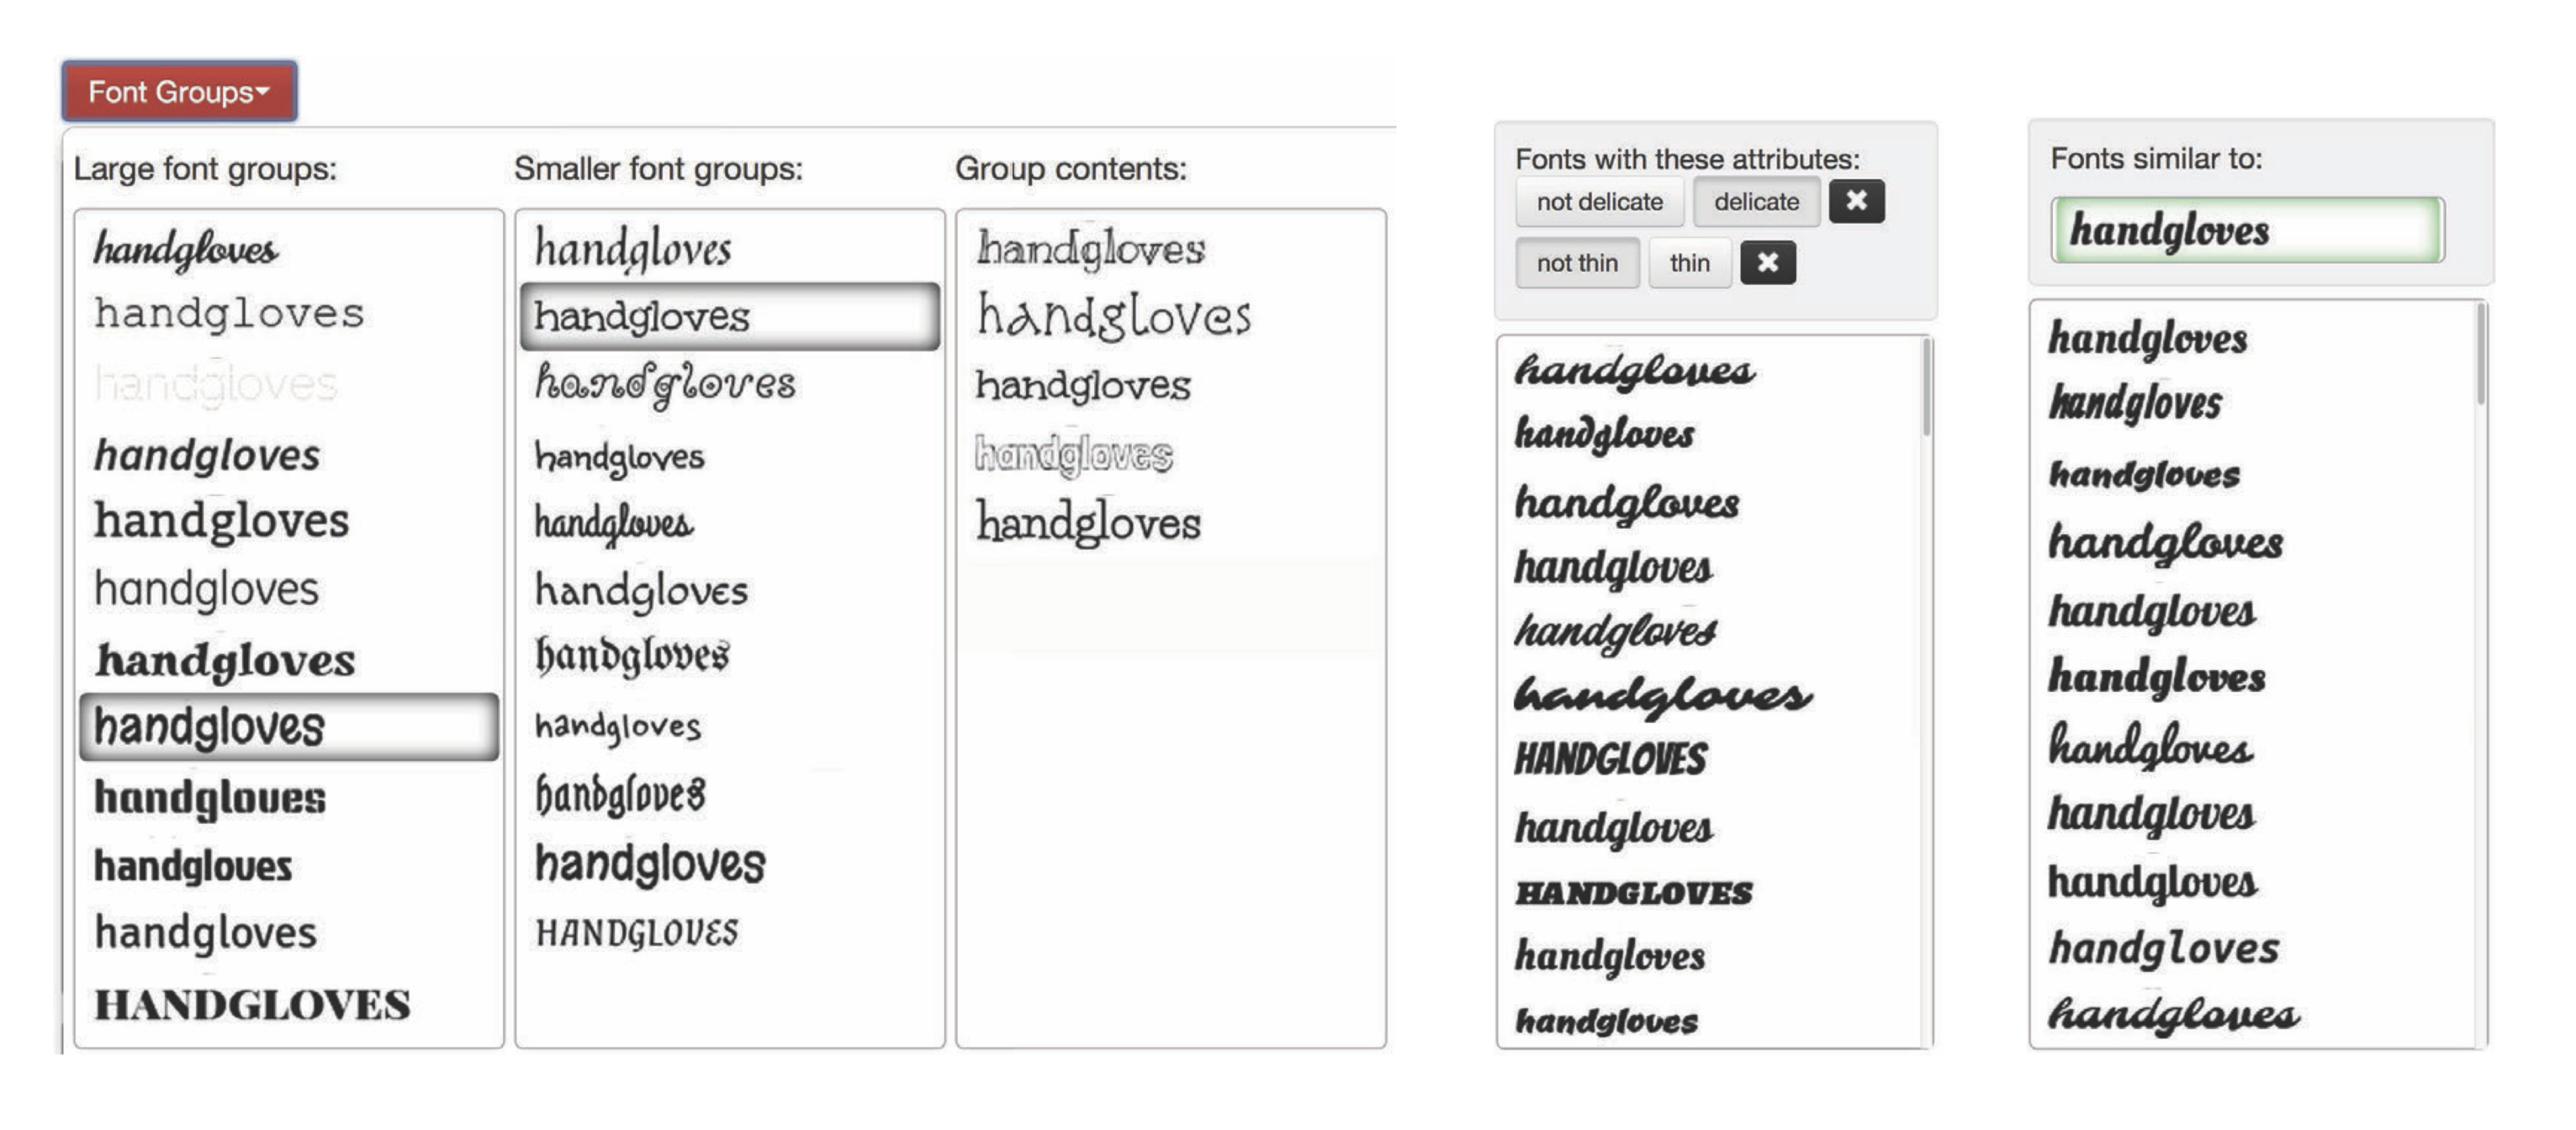
\includegraphics[width=1\textwidth]{images/odonovan-interfaces.png}
    \caption{Group Interface, Attribute Interface, and Search-By-Similarity selection tools from O'Donovan et al.}
    \label{fig:odonovan-interfaces}
\end{figure}

\subsection{Inference Models}

There has also been some effort to build inference models around font character images, often with the explicit purpose of building better user-interface for font selection. Cho et al. \cite{cho2022}, for example, builds a model with the explicit goal of generating latent space encodings of glyphs which are easily differentiable based on their font. They write:

\begin{quote}
    For the discriminative representation of a font from others, we propose a paired-glyph matching-based font representation learning model that attracts the representations of glyphs in the same font to one another, but pushes away those of other fonts.
\end{quote}

\begin{figure}[htbp]
    \centering
    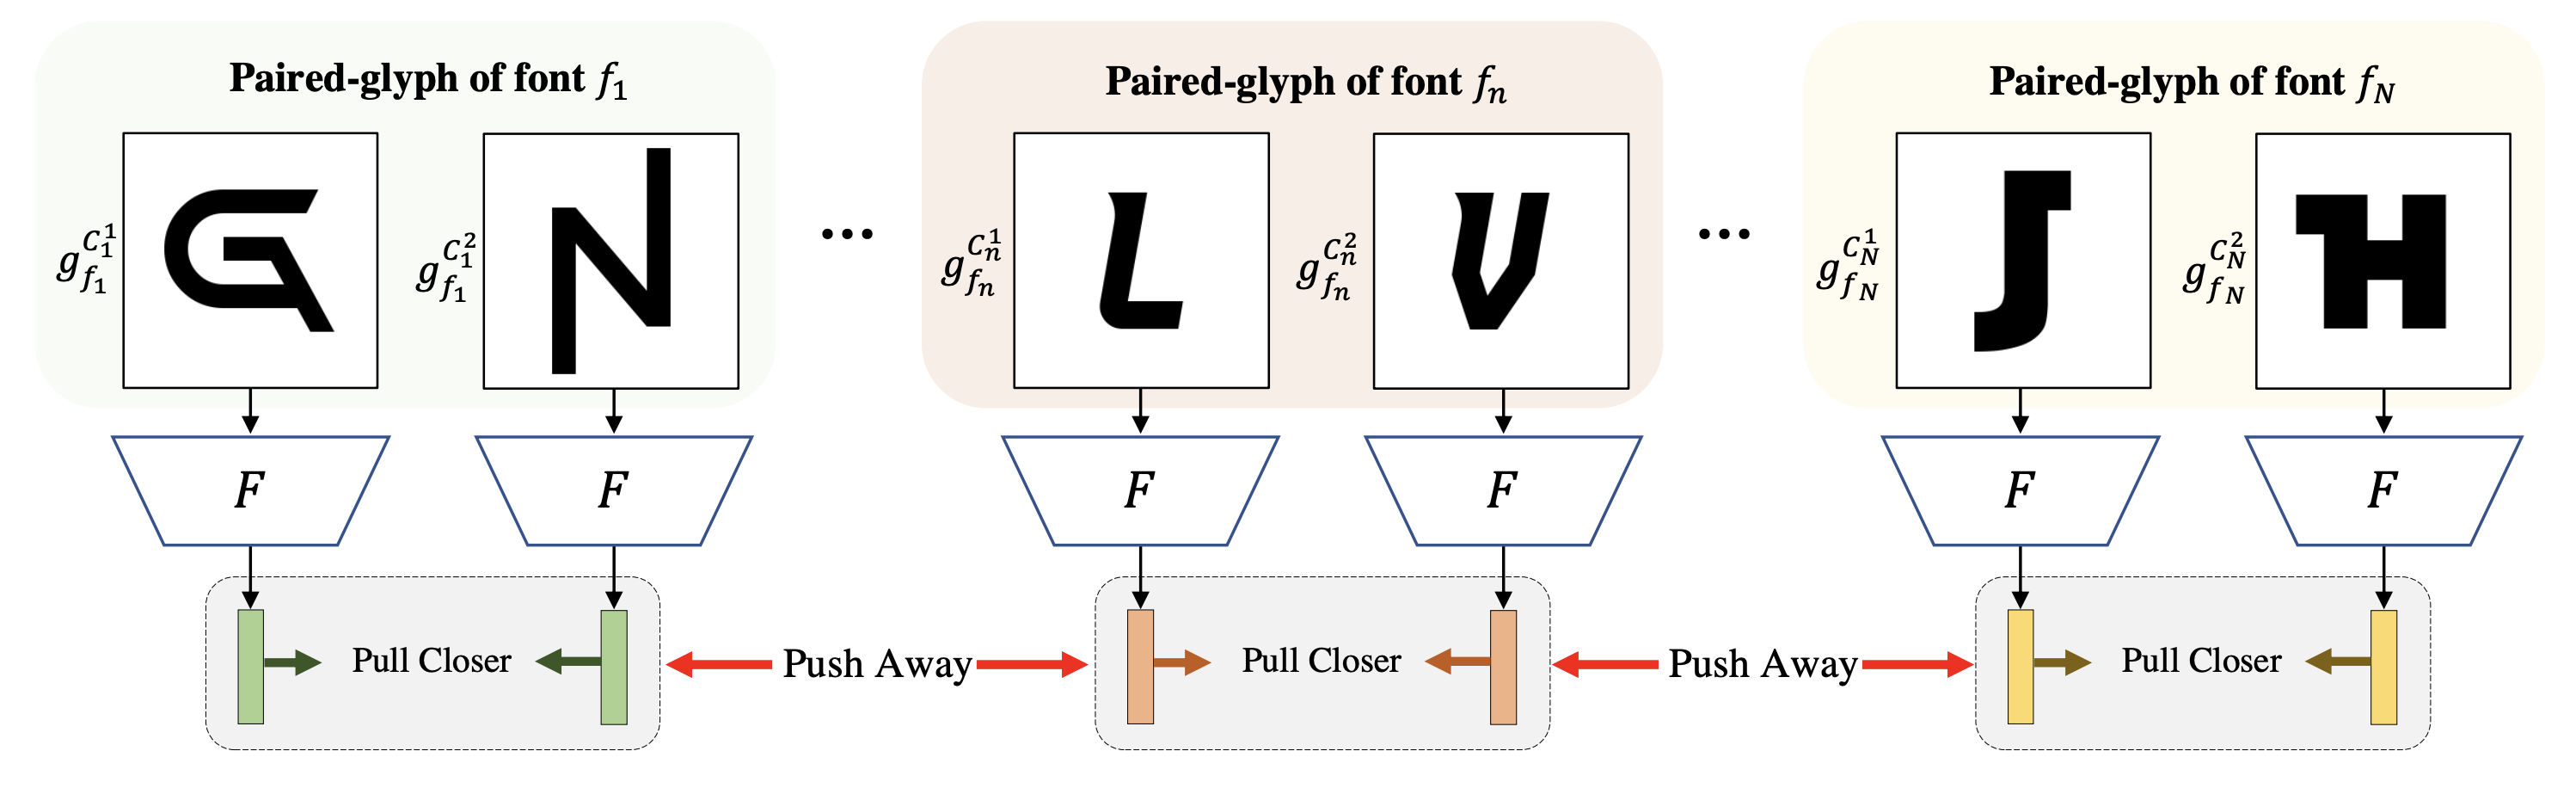
\includegraphics[width=1\textwidth]{images/cho-paired-glyph.png}
    \caption{Paired-glyph matching in Cho et al.}
    \label{fig:cho-paired-glyph}
\end{figure}

Their paired-glyph matching involves selecting random pairs of glyphs and training the model to prefer a low cosine similarity (more similar) between the representations if the glyphs are characters in the same font, and a high cosine similarity (less similar) if the glyphs come from different fonts. While Cho et al. succeeds in their goal of clustering the latent space representations of glyphs by typeface, we are skeptical of their methodology: by training the model to explicitly minimize cosine similarity between characters of the same typeface, it is unlikely that the resulting style encodings will generalize past the training data. Moreover, while two characters of the same font will have similar style encodings, it seems unlikely that the model will create a meaningful style encoding \textit{space.} The model may perform well in font discrimination tasks, but the model may not be encoding anything meaningful about the typefaces (style, weight, size) in the encodings which it produces.

\begin{figure}[b]
    \centering
    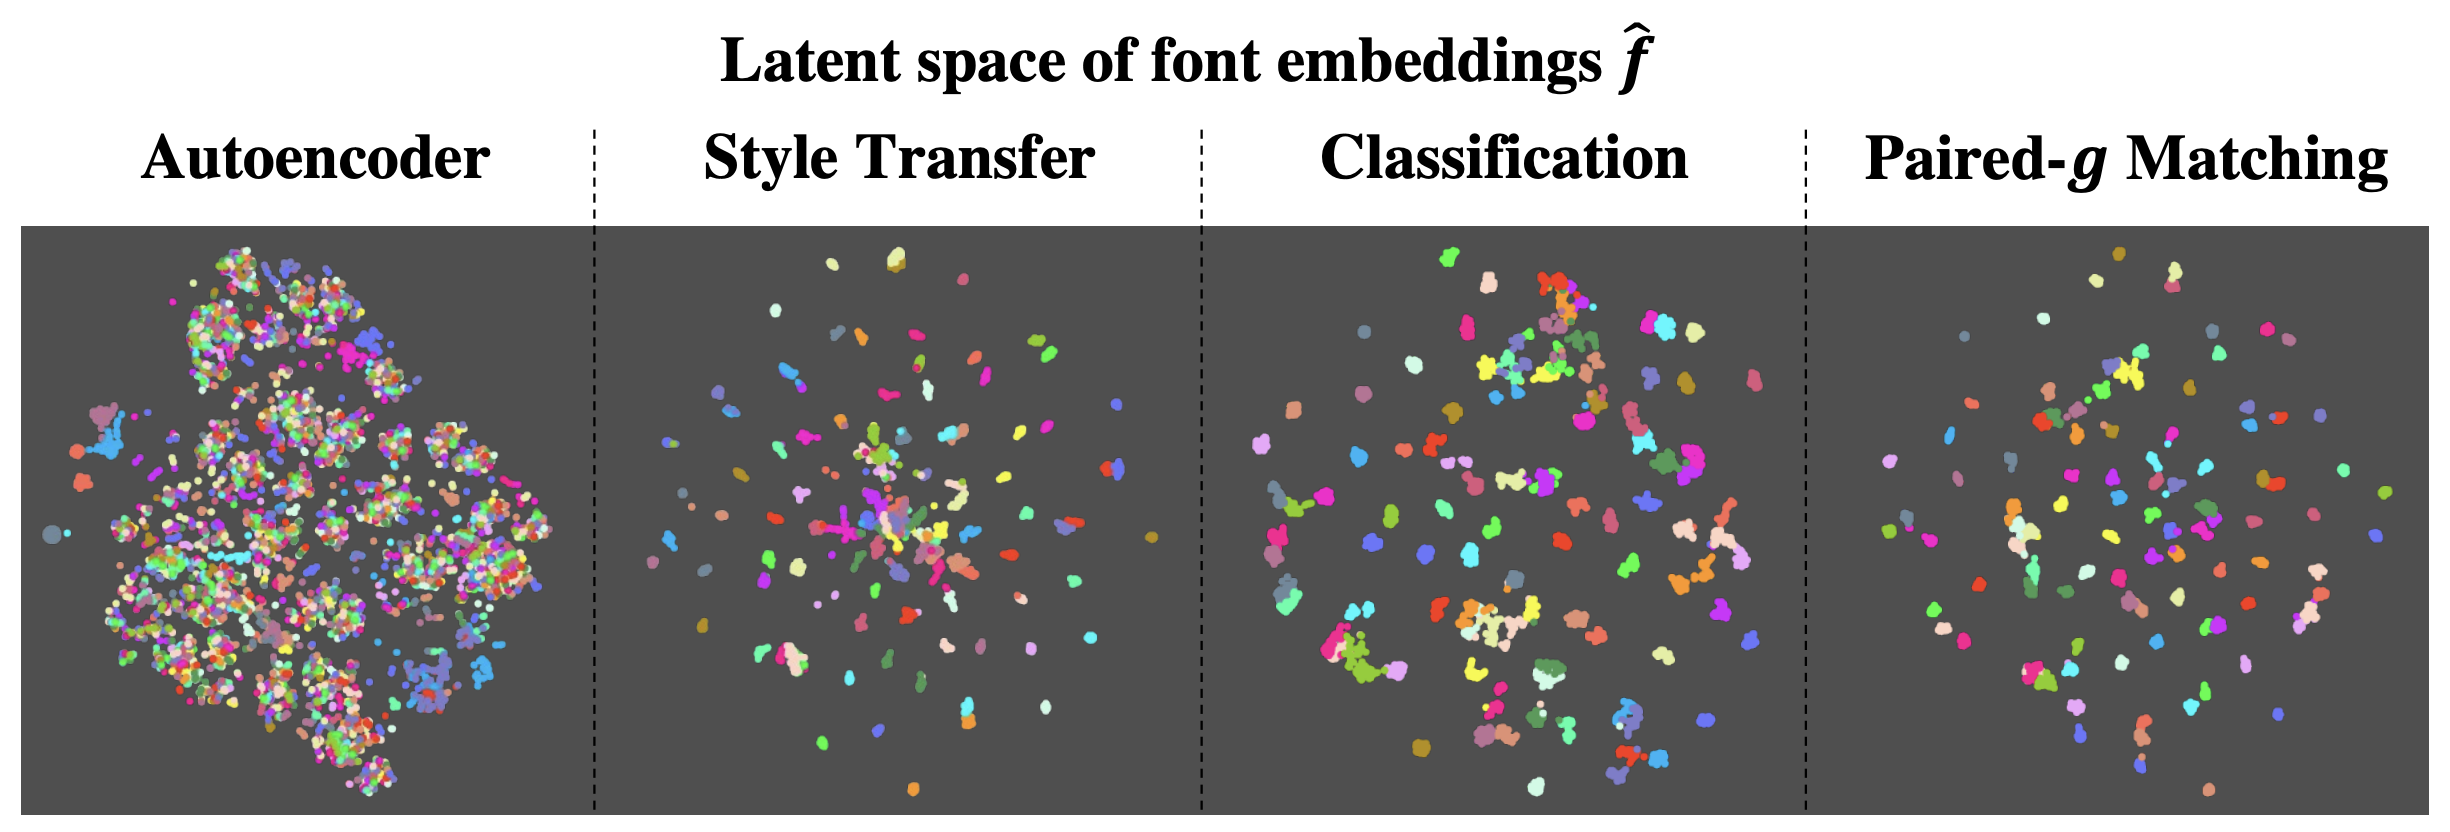
\includegraphics[width=1\textwidth]{images/cho-latent-space.png}
    \caption{Latent space of font embeddings across model techniques in Cho et al.}
    \label{fig:cho-latent-space}
\end{figure}

One aspect of Cho et al. which is helpful for our work is the set of model techniques they test. As shown in the latent space maps in Figure \ref{fig:cho-latent-space}, they employ three different model architectures in addition to their paired-glyph matching: the basic autoencoder model, style transfer (generating another character in the same font given an input character), and classification (predicting which font is represented in a glyph). There is an overlap in some of their model choices and ours (namely, autoencoder and style transfer), and their figure is also useful in visualizing the typeface-clustering effectiveness of these various models.

\begin{figure}[H]
    \centering
    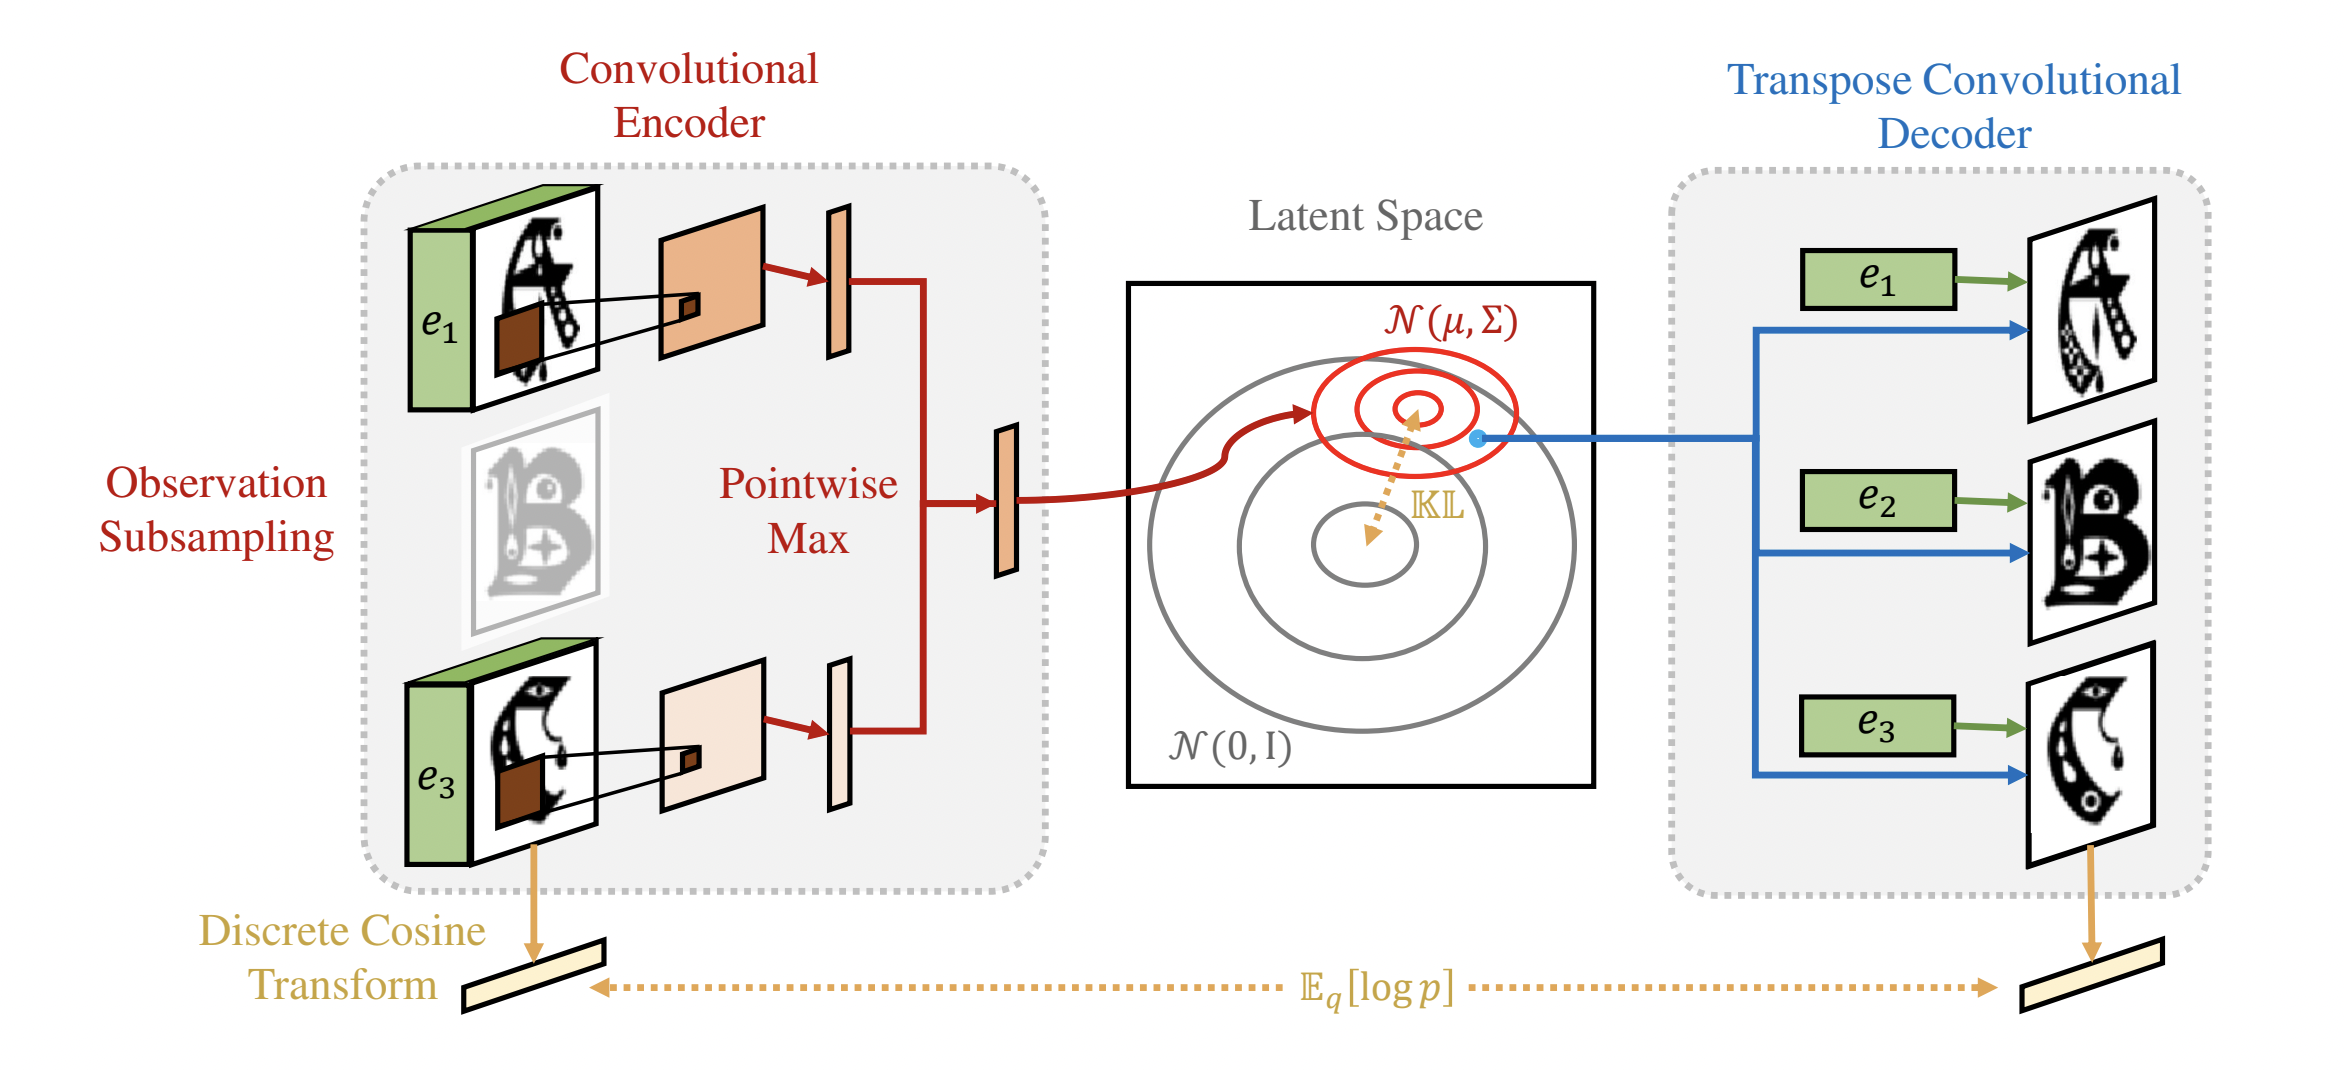
\includegraphics[width=1\textwidth]{images/srivatsan-model.png}
    \caption{Generative process of model Srivatsan et al.}
    \label{fig:srivatsan-model}
\end{figure}

Srivatsan et al. \cite{srivatsan2020} introduces an exciting novel training method based on latent probability space and a tensor factorization approach well-founded in past literature. Their model explicitly seeks to disentangle style and content—to encode font style as separate from the actual character it represents. The model architecture, shown in Figure \ref{fig:srivatsan-model}, convolutionally encodes a probabilistic embedding of a font given its complete character glyph set (with a chosen number missing) and corresponding character embeddings, and uses that latent probability vector along with a given character embedding to reconstruct the missing glyphs. Their model is particularly effective at reconstructing glyphs, when compared to peer models, and it also succeeds against a state-of-the-art peer model when evaluated by humans on Amazon Mechanical Turk. Figure \ref{fig:srivatsan-latent} shows a t-SNE projection of their model latent space with ``A'' glyphs displayed at each centroid given k-means clustering ($k=10$). Srivatsan et al. additionally find that, qualitatively, their model effectively recreates many important aspects of character style.

\begin{figure}
    \centering
    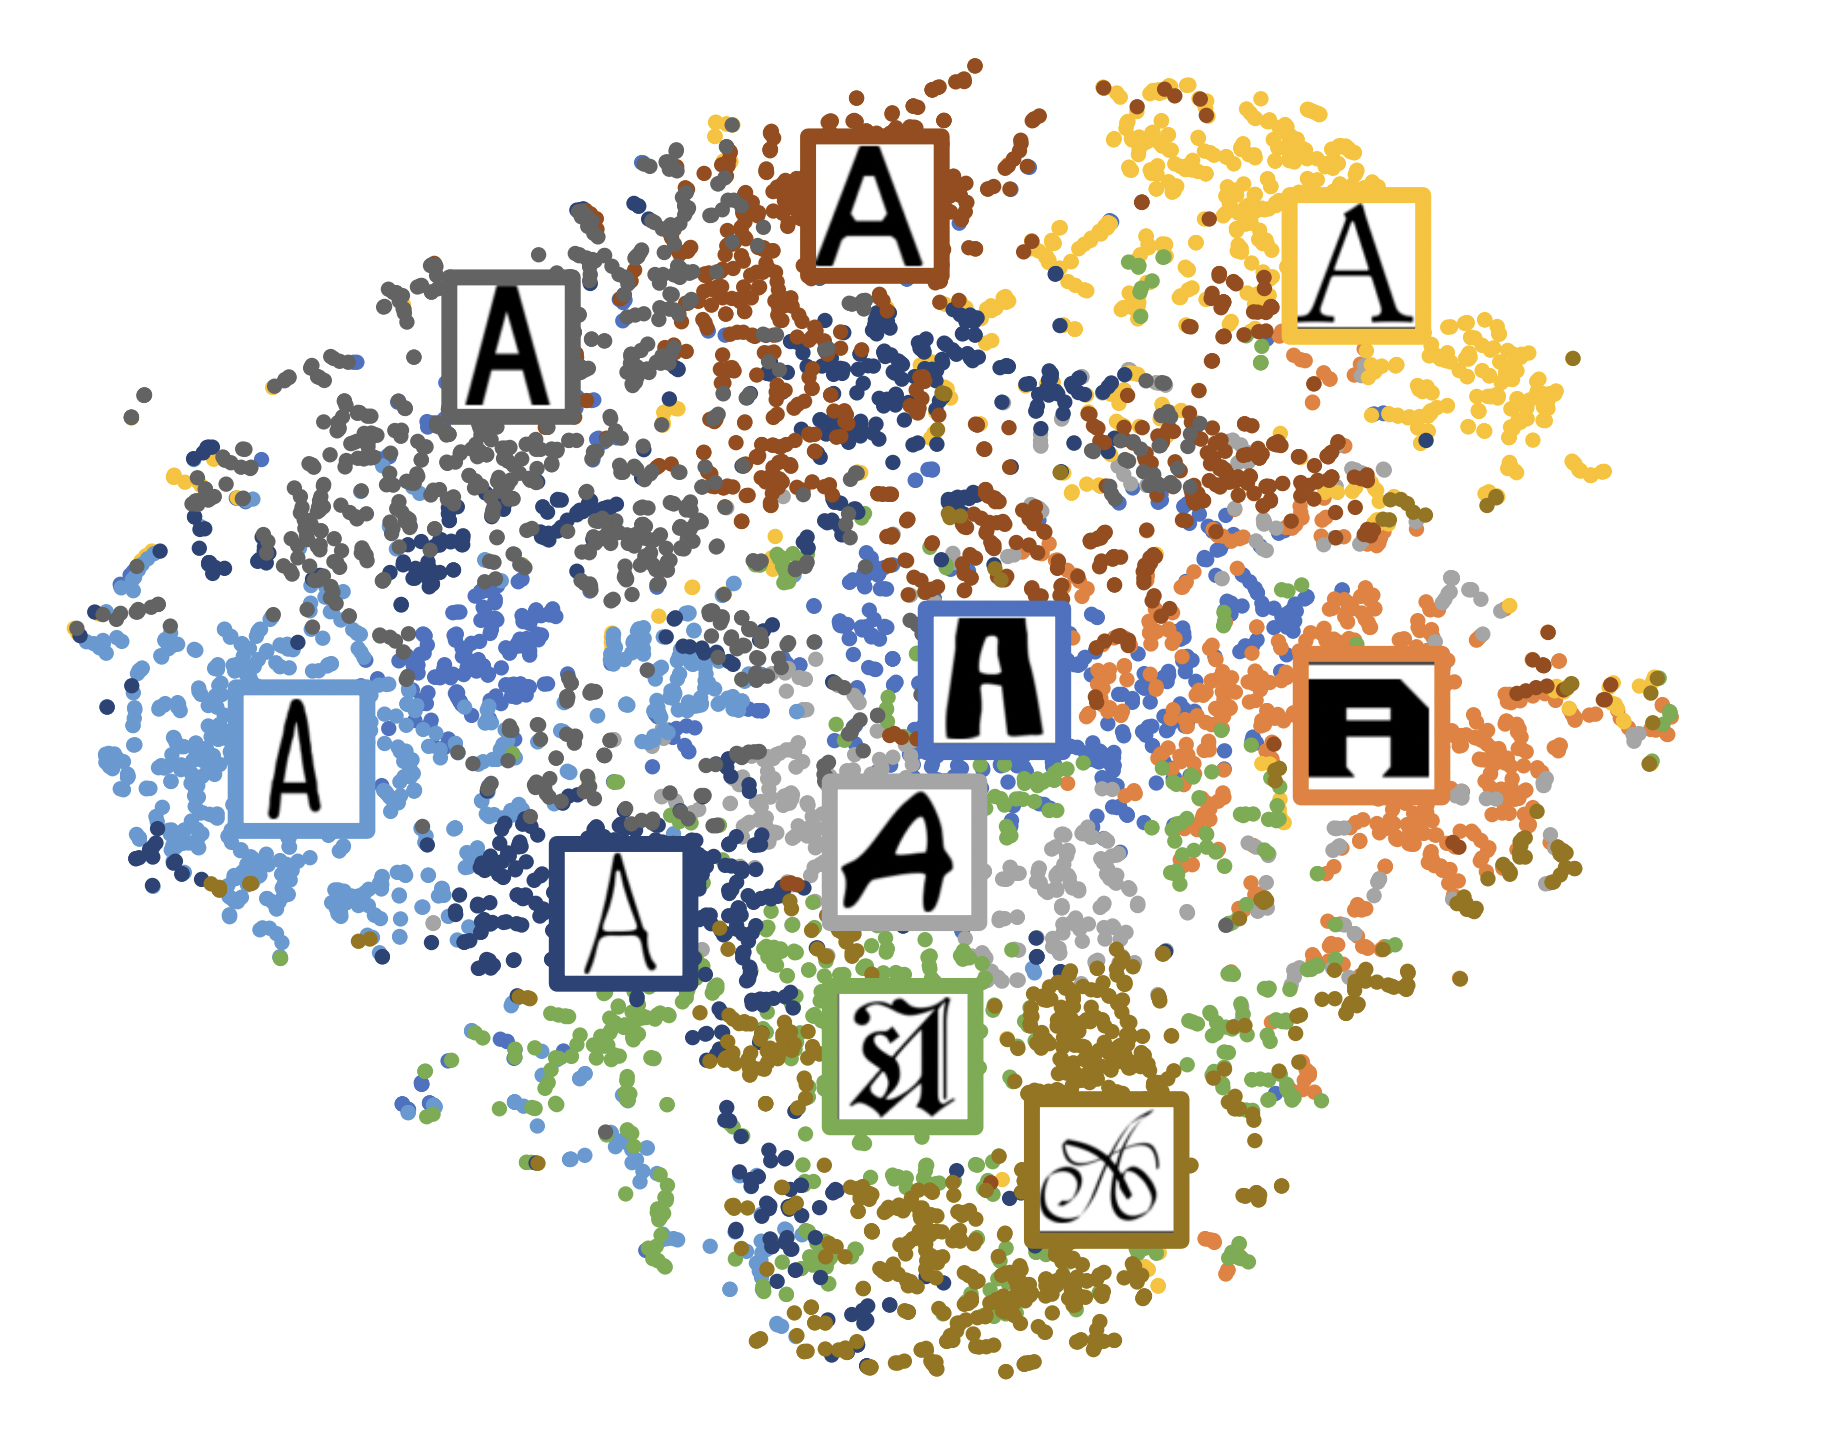
\includegraphics[width=.6\textwidth]{images/srivatsan-latent.png}
    \caption{t-SNE projection of latent font variables in Srivatsan et al. with centroids}
    \label{fig:srivatsan-latent}
\end{figure}